\documentclass[12pt,a4paper,leqno]{report}

\usepackage[UTF8]{inputenc}
\usepackage[T1]{fontenc}
\usepackage[finnish]{babel}
\usepackage{amsthm}
\usepackage{amsfonts}         
\usepackage{amsmath}
\usepackage{amssymb}
\usepackage{graphicx}
\usepackage{array}
\usepackage{hyperref}
\usepackage{rotating}

\pagestyle{plain}
\setcounter{page}{1}
\addtolength{\hoffset}{-1.15cm}
\addtolength{\textwidth}{2.3cm}
\addtolength{\voffset}{0.45cm}
\addtolength{\textheight}{-0.9cm}

\title{Tietokantasovellus: Keskustelufoorumi (dokumentaatio)}
\author{Wille Lehtomäki}
\date{}

\begin{document}

\maketitle

\tableofcontents

\chapter{Johdanto}\label{johd}

Työssä toteutetaan PHP-kielellä keskustelufoorumi, jonka käyttämiseen (siis pelkkään lukemiseenkin) tarvitaan käyttäjätunnus. Lisäksi yksittäisille keskustelualueille voi asettaa lukuoikeusrajoituksia, jolloin vain tiettyihin käyttäjäryhmiin kuuluvat käyttäjät voivat lukea niitä. Foorumiln ylläpitäjät voivat tavallisen käyttäjän oikeuksien lisäksi myös esimerkiksi poistaa viestejä ja lisätä aihekategorioita ja käyttäryhmiä.

Foorumi käyttää PostgreSQL-tietokantaa. Tietokannan vaihtaminen edellyttää ohjelmakoodin muokkaamista.

\chapter{Yleiskuva järjestelmästä}

\begin{center}
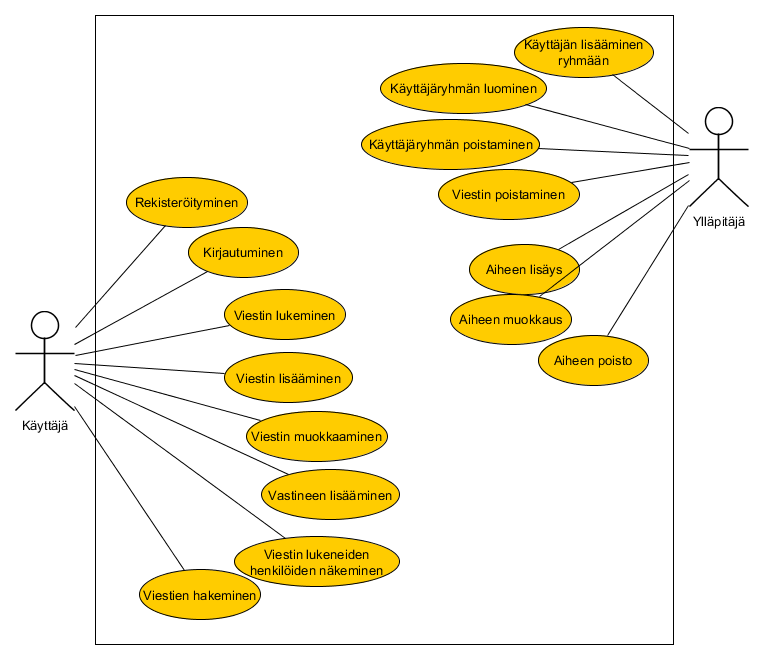
\includegraphics[scale=0.5]{kayttp}
\end{center}

\noindent \textbf{Huom:} Ylläpitäjä voi tehdä kaikki samat asiat kuin Käyttäjäkin, mutta luettavuuden vuoksi nämä yhteydet on jätetty kaaviossa merkitsemättä.

\Large\textbf{Käyttäjäryhmät}\normalsize\\

\emph{Käyttäjä} on foorumin ns. "tavallinen"  käyttäjä, eli henkilö, joka voi esimerkiksi lukea ja kirjoittaa viestejä.\\

Foorumin \emph{ylläpitäjällä} on lisäksi oikeus mm. poistaa viestejä ja määritellä viesteille aihealueita niiden järjestelemiseksi sekä hallita käyttäjäryhmiä.\\ \\

\Large\textbf{Käyttötapauskuvauksia}\normalsize\\

\textbf{Viestin lisääminen}

\noindent Käyttäjä kirjoittaa ja lisää foorumille uuden aloitusviestin, eli viestin, joka ei ole vastine mihinkään vanhaan viestiin. Muut käyttäjät voivat sekä lukea viestin että kirjoittaa sille vastineita.\\

\textbf{Vastineen lisääminen}

\noindent Vastine on vastausviesti johonkin aiemmin kirjoitettuun viestiin.\\

\textbf{Viestin lukeneiden näkeminen}

\noindent Käyttäjälle näytetään lista kaikista käyttäjistä, jotka ovat lukeneet tietyn viestin.\\

\textbf{Viestien hakeminen}

\noindent Viestejä voi hakea kirjoittajan, aiheen tai kirjoituspäivän perusteella.\\

\textbf{Viestin poistaminen}

\noindent Ylläpitäjä voi poistaa joko yksittäisiä vastineita tai kokonaisen viestiketjun poistamalla ketjun aloitusviestin.\\

\textbf{Käyttäjäryhmän luominen}

\noindent Ylläpitäjä voi luoda käyttäjille ryhmiä.\\

\textbf{Aiheen lisäys}

\noindent Käyttäjien ryhmittelyn lisäksi ylläpitäjä voi ryhmitellä myös viestejä asettamalla viesteille eri aihealueita, joihin kukin viesti mahdollisine vastineineen kuuluu.\\

\noindent Loput käyttötapaukset on listattu käyttötapauskaaviossa.

\chapter{Järjestelmän tietosisältö}

\begin{center}
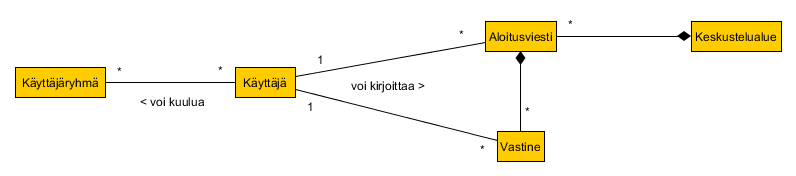
\includegraphics[scale=0.55]{tietosisaltokaavio}
\end{center}

\renewcommand{\arraystretch}{1.5}

\noindent \textbf{Käyttäjäryhmä}

\begin{center}
\begin{tabular}{| l | l | l | l |}
\hline
\textbf{Attribuutti} & \textbf{Arvojoukko} & \textbf{Kuvaus} \\ \hline
Tunnus & Kokonaisluku & Käyttäjäryhmän yksilöivä tunnus \\ \hline
Nimi & Merkkijono, max 30 merkkiä & Käyttäjäryhmän nimi \\ \hline
\end{tabular}
\end{center}
\ \\

\noindent \textbf{Käyttäjä}

\begin{center}
\begin{tabular}{| l | l | l | l |}
\hline
\textbf{Attribuutti} & \textbf{Arvojoukko} & \textbf{Kuvaus} \\ \hline
Tunnus & Kokonaisluku & Käyttäjän yksilöivä tunnus \\ \hline
Käyttäjätunnus & Merkkijono, max 30 merkkiä & Käyttäjän käyttäjätunnus \\ \hline
Salasana & Merkkijono, max 20 merkkiä & Käyttäjän salasana (selkokielinen) \\ \hline
\end{tabular}
\end{center}
\ \\ \\

 \noindent \textbf{Aloitusviesti}

\begin{center}
\begin{tabular}{| l | l |m{0.3\linewidth}|}
\hline
\textbf{Attribuutti} & \textbf{Arvojoukko} & \textbf{Kuvaus} \\ \hline
Tunnus & Kokonaisluku & Viestin yksilöivä tunnus \\ \hline
Kirjoittaja & Kokonaisluku & Viestin kirjoittaneen käyttäjän id \\ \hline
Keskustelualue & Merkkijono, max 50 merkkiä & Mihin keskustelualueeseen viesti kuuluu \\ \hline
Sisältö & Merkkijono, max 65 535 merkkiä & Viestin sisältö \\ \hline
Otsikko & Merkkijono, max 30 merkkiä & Viestin otsikko \\ \hline
Päivämäärä & Päivämäärä & Viestin kirjoituspäivämäärä \\ \hline
\end{tabular}
\end{center}
\ \\

\noindent \textbf{Vastine}

\begin{center}
\begin{tabular}{| l | l |m{0.3\linewidth}|}
\hline
\textbf{Attribuutti} & \textbf{Arvojoukko} & \textbf{Kuvaus} \\ \hline
Tunnus & Kokonaisluku & Vastineen yksilöivä tunnus \\ \hline
Kirjoittaja & Kokonaisluku & Viestin kirjoittaneen käyttäjän id \\ \hline
Aloitusviesti & Kokonaisluku & Sen viestin tunnus, johon vastine on vastaus \\ \hline
Sisältö & Merkkijono, max 65 535 merkkiä & Vastineen sisältö \\ \hline
Päivämäärä & Päivämäärä & Vastineen kirjoituspäivämäärä \\ \hline
\end{tabular}
\end{center}
\ \\ \\ \\ \\

\noindent \textbf{Keskustelualue}

\begin{center}
\begin{tabular}{| l | l | l | l |}
\hline
\textbf{Attribuutti} & \textbf{Arvojoukko} & \textbf{Kuvaus} \\ \hline
Tunnus & Kokonaisluku & Keskustelualueen yksilöivä tunnus \\ \hline
Nimi & Merkkijono, max 50 merkkiä & Keskustelualueen nimi \\ \hline
\end{tabular}
\end{center}

\chapter{Relaatiotietokantakaavio}

\begin{center}
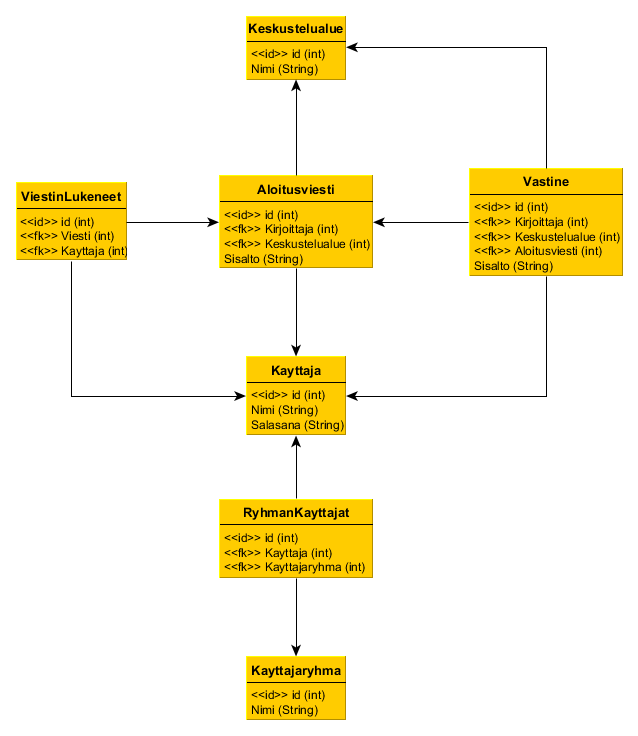
\includegraphics[scale=0.55]{relaatiotietokantakaavio}
\end{center}

\chapter{Järjestelmän yleisrakenne}

Työ noudattaa MVC-mallia, mutta kaikki kontrollerit (apukontrollereineen) on sijoitettu projektin juureen. Yleiskäyttöiset, lähinnä istuntoa koskevat apufunktiot on sijoitettu libs-kansion funtkiot.php-tiedostoon.

Näkymät puolestaan ovat views-kansiossa, ja mallit libs-kansion alikansiossa models (malliluokkien tiedostonimet on kirjoitettu isolla alkukirjaimella).

Vain kirjautumis- ja rekisteröitymissivuja on mahdollista tarkastella kirjautumatta sisään. Ylläpitoalueen sivut puolestaan ovat vain ylläpitäjien nähtävissä.

\chapter{Käyttöliittymä ja järjestelmän komponentit}

Sivukartta (seuraavalla sivulla):

\begin{sideways}
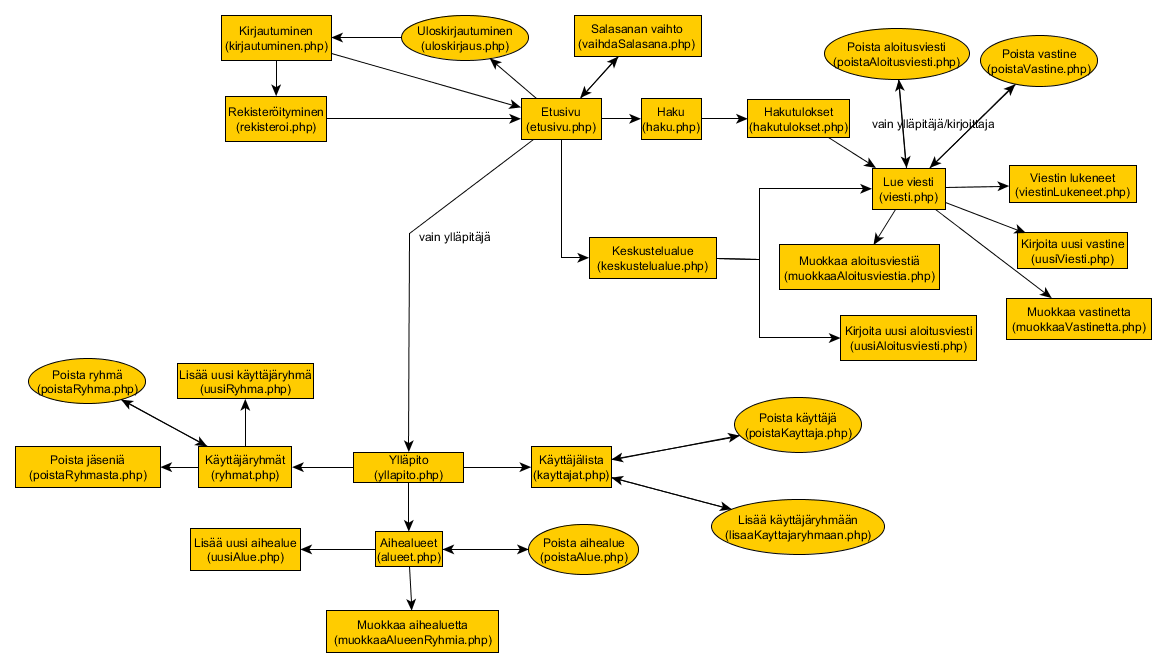
\includegraphics[scale=.55]{sivukartta}
\end{sideways}

\chapter{Asennustiedot}

Kopioi tiedostot palvelimelle. Oletusarvoisesti (add-test-data.sql-tiedostossa määritellysti) foorumin ylläpitäjän käyttäjätunnus on Teppo ja salasana kappelo. Koska foorumi tallentaa salasanat selkokielisesti (ja salasana on näkyvissä yllämainitussa tiedostossa), kannattaa salasana vaihtaa heti ensikirjautumisen jälkeen sovelluksen Vaihda salasana -välilehdeltä.

Sovelluksella ei ole erillistä asetustiedostoa.

\chapter{Käynnistys- / käyttöohje}

Normaalin käyttäjän tunnus ja salasana: Tapsa, koppelo\\
Ylläpitäjän tunnus ja salasana: Teppo, kappelo\\

\noindent Foorumille on myös mahdollista tehdä oma käyttäjätunnus.\\

\noindent Linkkejä:\\
\href{http://wlehtoma.users.cs.helsinki.fi/Keskustelufoorumi/esittelysivu.html}{Esittelysivu}\\
\href{http://wlehtoma.users.cs.helsinki.fi/Keskustelufoorumi/html-demo/}{Html-demo}\\
\href{http://wlehtoma.users.cs.helsinki.fi/Keskustelufoorumi/kirjautuminen.php}{Foorumi}

\chapter{Testaus, tunnetut bugit ja puutteet \& jatkokehitysideat}

Hakutoiminto on hyvin alkeellinen. Lisäksi hakutulokset näyttävällä sivulla ei ole sivutusta, joten hakutuloksien määrästä riippumatta tulokset näytetään samalla sivulla.  \\

\noindent Järjestelmä tallentaa salasanat selkokielisenä, mikä ei ole paras mahdollinen ratkaisu.\\

\noindent Testaus on suoritettu manuaalisesti.

\chapter{Omat kokemukset}

En ollut aiemmin käyttänyt PHP:tä, joten ongelmia ja päänvaivaa riitti. Esimerkiksi GET- ja POST-parametrit olivat jostain syystä mysteeri pitkän aikaa.\\

\noindent Kuten muillakin kursseilla, dokumentaation räpeltäminen oli aina kurssin kuivinta antia. Ja itse kurssi oli yllättävän työläs, mutta tulipahan opittua PHP:tä.

\end{document}